\documentclass{article}
\usepackage[utf8]{inputenc}
\usepackage[spanish]{babel}
\usepackage{enumitem}
\usepackage{amssymb}
\usepackage{listingsutf8}
\usepackage{amsmath}
\usepackage{geometry}
\usepackage[outline]{contour}
\usepackage[dvipsnames]{xcolor}
\geometry{tmargin=2cm, lmargin=2.5cm, rmargin=2.5cm, bmargin=2cm}
\usepackage{tikz}
\usepackage{xcolor}

\usepackage{blindtext}

\usepackage{hyperref}

\lstset{
    inputencoding=utf8,
    extendedchars=true,
    literate={á}{{\'a}}1 {é}{{\'e}}1 {í}{{\'i}}1 {ó}{{\'o}}1 {ú}{{\'u}}1 {ñ}{{\~n}}1
}

\hypersetup{
    colorlinks=true,
    linkcolor=blue,
    filecolor=magenta,      
    urlcolor=cyan,
    }
    
\urlstyle{same}

\definecolor{codegreen}{rgb}{0,0.6,0}
\definecolor{codegray}{rgb}{0.5,0.5,0.5}
\definecolor{codepurple}{rgb}{0.58,0,0.82}
\definecolor{backcolour}{rgb}{0.95,0.95,0.92}

\lstdefinestyle{mystyle}{
  backgroundcolor=\color{backcolour}, commentstyle=\color{codegreen},
  keywordstyle=\color{magenta},
  numberstyle=\tiny\color{codegray},
  stringstyle=\color{codepurple},
  basicstyle=\ttfamily\footnotesize,
  breakatwhitespace=false,         
  breaklines=true,                 
  captionpos=b,                    
  keepspaces=true,                 
  numbers=left,                    
  numbersep=5pt,                  
  showspaces=false,                
  showstringspaces=false,
  showtabs=false,                  
  tabsize=2
}
\lstset{style=mystyle}

\title{Universidad Nacional Autónoma de México \\\bigskip Facultad de Ciencias \\\bigskip Riesgo Tecnológico 2025-1 \\\bigskip \textbf{Laboratorio: Histogramas}}

\author{\textbf{Profesora:} \\\bigskip Selene Marisol Martínez Ramírez \\\bigskip \textbf{Ayudantes:} \\\bigskip  César Eduardo Jardines Mendoza \\\bigskip Itzel Azucena Delgado Díaz \\\bigskip Luis Angel Rojas Espinoza \\\bigskip Luis Rey Rutiaga Robles \\\bigskip \textbf{INTEGRANTES:} \\\bigskip Deloya Andrade Ana Valeria \\\bigskip Cortés Jiménez Carlos Daniel \\\bigskip Cruz Gonzalez Irvin Javier \\\bigskip Castro Reyes Angel \\\bigskip Cruz Blanco Gabriela}

\begin{document}

\maketitle

\newpage
 
\section{Histogramas}

\begin{itemize}
    \item \textbf{Histograma del monto de las transacciones por hora del día con estado fraudolento de nuevos usuarios (Cuanto dinero históricamente se ha perdido más en las 24 horas del día):}

        A continuación se muestra la implementación de este histograma, para ejecutarlo basta con colocar en terminal el comando \textbf{python3 histograma1.py}:

        \begin{lstlisting}[language=Python, caption=Implementación del Histograma del monto de transacciones por hora del día]
            import pandas as pd
            import matplotlib.pyplot as plt
            import seaborn as sns
            import matplotlib.patches as mpatches
            
            # Cargar el archivo CSV
            data = pd.read_csv('transacciones.csv')
            
            # Crear una nueva columna combinando 'date' y 'time'
            data['transaction_time'] = pd.to_datetime(data['date'] + ' ' + data['time'], format='%d/%m/%Y %H:%M')
            
            # Filtrar para obtener solo transacciones fraudulentas de nuevos usuarios
            fraudulent_transactions_new_users = data.loc[(data['status'] == 'fraudulent') & (data['new_user'] == True)].copy()
            
            # Extraer la hora del día de la columna 'transaction_time'
            fraudulent_transactions_new_users.loc[:, 'hour'] = fraudulent_transactions_new_users['transaction_time'].dt.hour
            
            # Añadimos un estilo a la gráfica
            sns.set(style="whitegrid")
            
            # Se define y se crea la gráfica
            plt.figure(figsize=(10, 6))
            colors = ["#FF6F61"]
            
            # Crear el histograma con el monto por hora
            sns.histplot(
                data=fraudulent_transactions_new_users,
                x='hour', 
                weights='amount',  # Aquí el peso será el monto de la transacción
                bins=24,  # Una barra por cada hora del día
                color=colors[0],
                edgecolor='black'
            )
            
            # Títulos y etiquetas
            plt.title('Monto de transacciones fraudulentas por hora del día (nuevos usuarios)', fontsize=16, fontweight='bold')
            plt.xlabel('Hora del día', fontsize=14)
            plt.ylabel('Monto total de transacciones fraudulentas', fontsize=14)
            
            # Personalizamos los ejes
            plt.xticks(range(0, 24), fontsize=12)
            plt.yticks(fontsize=12)
            
            # Cuadrícula en la gráfica
            plt.grid(axis='y', linestyle='--', alpha=0.7)
            
            # Crear la leyenda "Fraudulentas"
            fraud_patch = mpatches.Patch(color='#FF6F61', label='Fraudulentas')
            
            # Guardar la gráfica como imagen en lugar de mostrarla
            plt.legend(handles=[fraud_patch], title='Estado', loc='upper right', fontsize=12)
            plt.tight_layout()
            
            # Guardar la gráfica en un archivo PNG
            plt.savefig('IMAGE/histograma1.png')
            
            plt.show()
        \end{lstlisting}

        El histograma es el siguiente:

        \begin{center}
            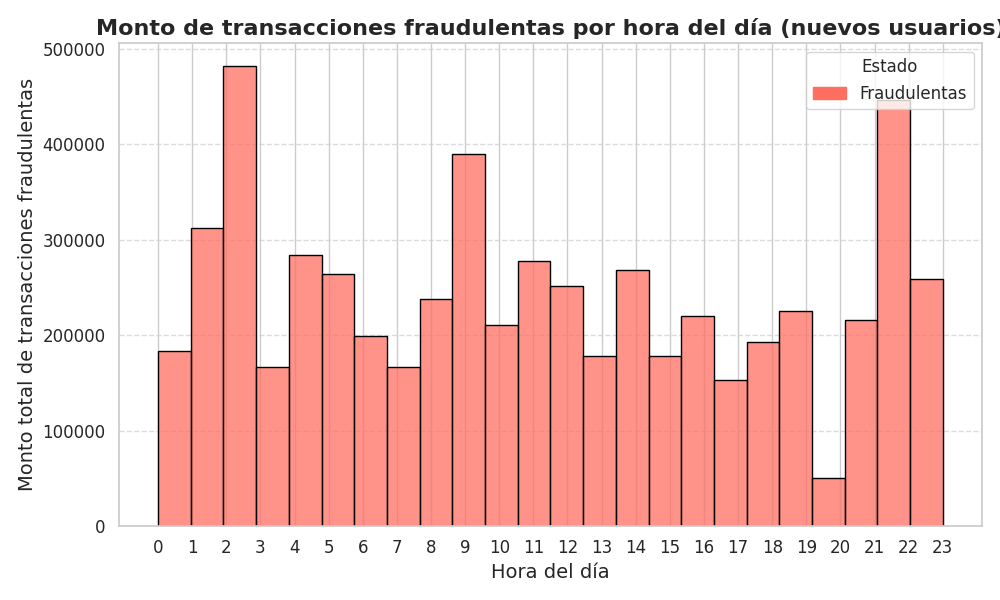
\includegraphics[scale=0.5]{IMAGE/histograma1.png}
        \end{center}

        Este histograma permite visualizar las horas en las que se realizan más transacciones fraudulentas en términos de monto, lo cual puede proporcionar información valiosa para ajustar las medidas de seguridad y monitorear con más detalle ciertas horas críticas del día.

        En términos de análisis de riesgos, si el histograma muestra un pico durante ciertas horas (por ejemplo, entre la medianoche y las 3:00 a.m.), puede indicar que los atacantes prefieren operar en esos momentos, lo que lleva a la implementación de controles adicionales durante esas horas.

    \item \textbf{Histograma de la distribución de nuevos usuarios con una transacción fraudolenta (Cuantos usuarios nuevos tuvieron una transacción fraudolenta vs los usuarios que no son nuevos):}

    A continuación se muestra la implementación de este histograma, para ejercutarlo basta con colocar en terminal el comando \textbf{python3 histograma2.py}:

    \begin{lstlisting}[language=Python, caption=Implementación de histograma de la distribución de nuevos usuarios con una transacción fraudolenta.]
        import pandas as pd
        import matplotlib.pyplot as plt
        import seaborn as sns
        import matplotlib.patches as mpatches
        
        # Cargar el CSV
        data = pd.read_csv('transacciones.csv')
        
        # Filtra para obtener solo transacciones fraudulentas
        fraudulent_transactions = data[data['status'] == 'fraudulent']
        
        # Formato para extraer la informacion para las columnas de los usuarios no nuevos y nuevos
        fraudulent_transactions_users = fraudulent_transactions[
            (fraudulent_transactions['new_user'] == True) | 
            (fraudulent_transactions['new_user'] == False)]
        
        # Se añade un estilo a la gráfica
        sns.set(style="whitegrid")
        
        # Se define y se crea la gráfica
        plt.figure(figsize=(10, 6)) 
        colors = ["#73a13f", "#73a13f"]
        
        # Personalizamos las barras
        sns.histplot(
            data=fraudulent_transactions_users, 
            x='new_user', 
            hue='new_user',  
            multiple='stack', 
            palette=colors,
            shrink=7.5,  
            edgecolor='black')
        
        # Titulos
        plt.title('Cantidad de transacciones fraudulentas por tipo de usuario', fontsize=16, fontweight='bold')
        plt.xlabel('Tipo de usuario', fontsize=14)
        plt.ylabel('Cantidad de transacciones fraudulentas', fontsize=14)
        
        # Perzonalizamos los ejes
        plt.xticks([0, 1], ['Non New', 'New'], fontsize=12) 
        plt.yticks(fontsize=12)
        
        # Cuadrícula en la gráfica 
        plt.grid(axis='y', linestyle='--', alpha=0.7)
        
        # Crear la leyenda "Fraudulentas" de Estado
        new_patch = mpatches.Patch(color='#73a13f', label='Fraudulentas')
        
        # Muestra la gráfica
        plt.legend(handles=[new_patch], title='Estado', loc='upper right', fontsize=12)
        plt.tight_layout()
        plt.show()
    \end{lstlisting}

    El histograma es el siguiente:

    \begin{center}
        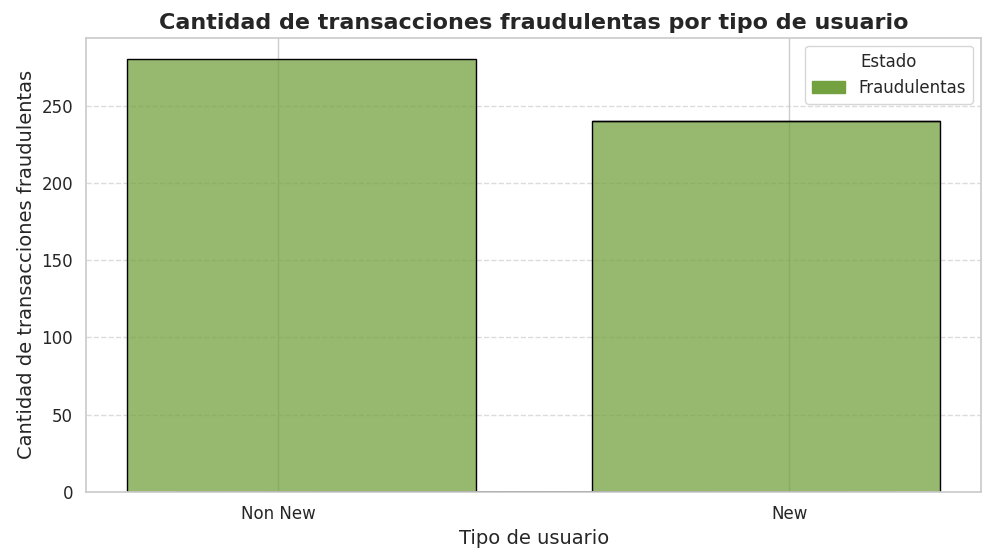
\includegraphics[scale = .4]{IMAGE/Histograma2.png}
    \end{center}

    Si bien hay una cantidad significativa de transacciones fraudolentas realizadas por los usuarios nuevos, existe una mayor cantidad realizada por aquellos usuarios que no son nuevos. Esto puede deberse a varios factores como que este sector de los usuarios tiene más experiencia y conocimiento en el manejo del sistema.

    Con la información recabada en este histograma puede tomarse medidas como la implementación de un mayor monitoreo y análisis del comportamiento en usuarios que ya llevan tiempo utilizando el servicio cuando estos llevan a cabo transacciones. Utilizando así los datos recabados para reforzar la seguridad del sistema de manera eficiente.

    \item \textbf{Histograma del tipo de transacción y el estado de la transacción fraudolenta (Cuántos estados de transacciones fraudolentas tuvieron las transacciones purchase y transfer):}

    El código usado fue el siguiente:

    \begin{lstlisting}[language=Python, caption=Implementación histograma del tipo de transacción y el estado de la transacción fraudolenta.]
    import pandas as pd
    import matplotlib.pyplot as plt
    import seaborn as sns
    import matplotlib.patches as mpatches

    # Cargar el CSV
    data = pd.read_csv('transacciones.csv')

    # Filtrar para obtener solo transacciones fraudulentas
    fraudulent_transactions = data[data['status'] == 'fraudulent']

    # Formato para extraer solo la compra y transfrencia de la columna 'purchase' y 'transfer'
    fraudulent_transactions_filtered = fraudulent_transactions[
        (fraudulent_transactions['transaction_type'] == 'purchase') | 
        (fraudulent_transactions['transaction_type'] == 'transfer')
    ]

    # Añadimos un estilo a la gráfica
    sns.set(style="whitegrid")

    #Se define y se crea la gráfica
    plt.figure(figsize=(10, 6)) 
    colors = ["#FF6F61", "#6B5B95"]

    # Personalizamos las barras
    sns.histplot(
        data=fraudulent_transactions_filtered, 
        x='transaction_type', 
        hue='status', 
        multiple='stack', 
        palette=colors,
        shrink=0.8,  
        edgecolor='black'  
    )

    #Titulos
    plt.title('Cantidad de transacciones fraudulentas por tipo de transacción', fontsize=16, fontweight='bold')
    plt.xlabel('Tipo de transacción', fontsize=14)
    plt.ylabel('Cantidad de transacciones fraudulentas', fontsize=14)

    # Perzonalizamos los ejes
    plt.xticks(fontsize=12)
    plt.yticks(fontsize=12)

    # Cuadrícula en la gráfica 
    plt.grid(axis='y', linestyle='--', alpha=0.7)

    # Crear la leyenda "Fraudulentas"
    fraud_patch = mpatches.Patch(color='#FF6F61', label='Fraudulentas')

    #Mostramos la gráfica
    plt.legend(handles=[fraud_patch], title='Estado', loc='upper right', fontsize=12)
    plt.tight_layout()
    plt.show()
    \end{lstlisting}

    También se adjuntara el archivo .py, abrimos nuestra terminal y ejecutamos \textbf{python3 histograma3.py} y la gráfica resultante es la siguiente:

    \begin{center}
        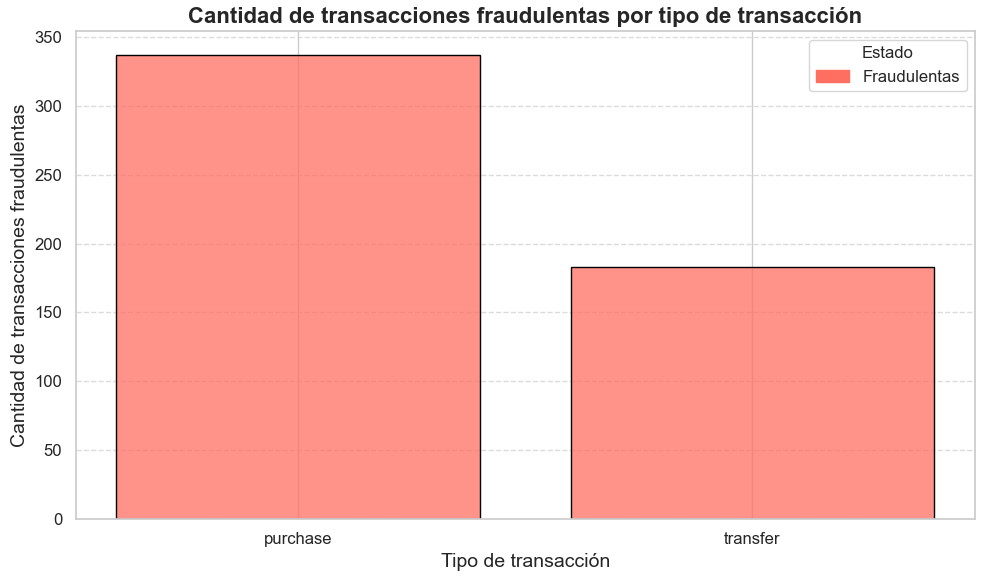
\includegraphics[scale = .4]{IMAGE/Histograma3.png}
    \end{center}

    Podemos ver que que la cantidad de transaccines de tipo ''purchase'' es más alta que las de ''transfer'',  esto nos puede decir que los sistemas de compra son mas propensos a que sean atacados, siendo que podría haber vulnerabilidades en la seguridad al realizar una compra y así haber menos control en esta área en comparación con las transferencias, por lo que los estafadores prefieren realizar fraudes mediante compras ya que les sería mas sencillo el poder realizar una acción fraudolenta entre las transacciones legítimas, ya que si realizan el fraude en transferencias esto pueder más fácil de rastrear.
\newpage
    \item \textbf{Histograma de los meses con transacciones fraudolentas:}

    A continuación se muestra la implementación de este histograma, para ejercutarlo basta con colocar en terminal el comando \textbf{python3 histograma5.py}:

      \begin{lstlisting}[language=Python, caption=Implementación histograma de los meses con transacciones fraudolentas.]
        import pandas as pd
        import matplotlib.pyplot as plt
        import seaborn as sns

        # Cargar los datos desde el archivo CSV
        data = pd.read_csv('transacciones.csv')

        # Filtrar para obtener solo transacciones fraudulentas
        fraudulent_transactions = data[(data['status'] == 'fraudulent')]

        # Formato para extraer solo el mes de la columna 'date'
        fraudulent_transactions['month'] = pd.to_datetime(fraudulent_transactions['date'], format='%d/%m/%Y').dt.month

        # Crear una lista de nombres de los meses
        months_names = ['Enero', 'Febrero', 'Marzo', 'Abril', 'Mayo', 'Junio', 'Julio', 'Agosto', 'Septiembre', 'Octubre', 'Noviembre', 'Diciembre']

        # Se define y se crea la gráfica con pesos
        plt.figure(figsize=(12, 6))  # Ajusta el tamaño de la figura
        sns.histplot(
         data=fraudulent_transactions, x='month', weights='amount', bins=12, kde=True, color='red', label='fraudulent')

        # Cambiar las etiquetas del eje X a los nombres de los meses
        plt.xticks(ticks=range(1, 13), labels=months_names)

        # Títulos
        plt.title('Distribución del monto de transacciones fraudulentas por mes del año')
        plt.xlabel('Mes del año')
        plt.ylabel('Monto')
        plt.grid(True)

        # Mostramos la gráfica
        plt.legend()
        plt.show()
    \end{lstlisting}

     \begin{center}
        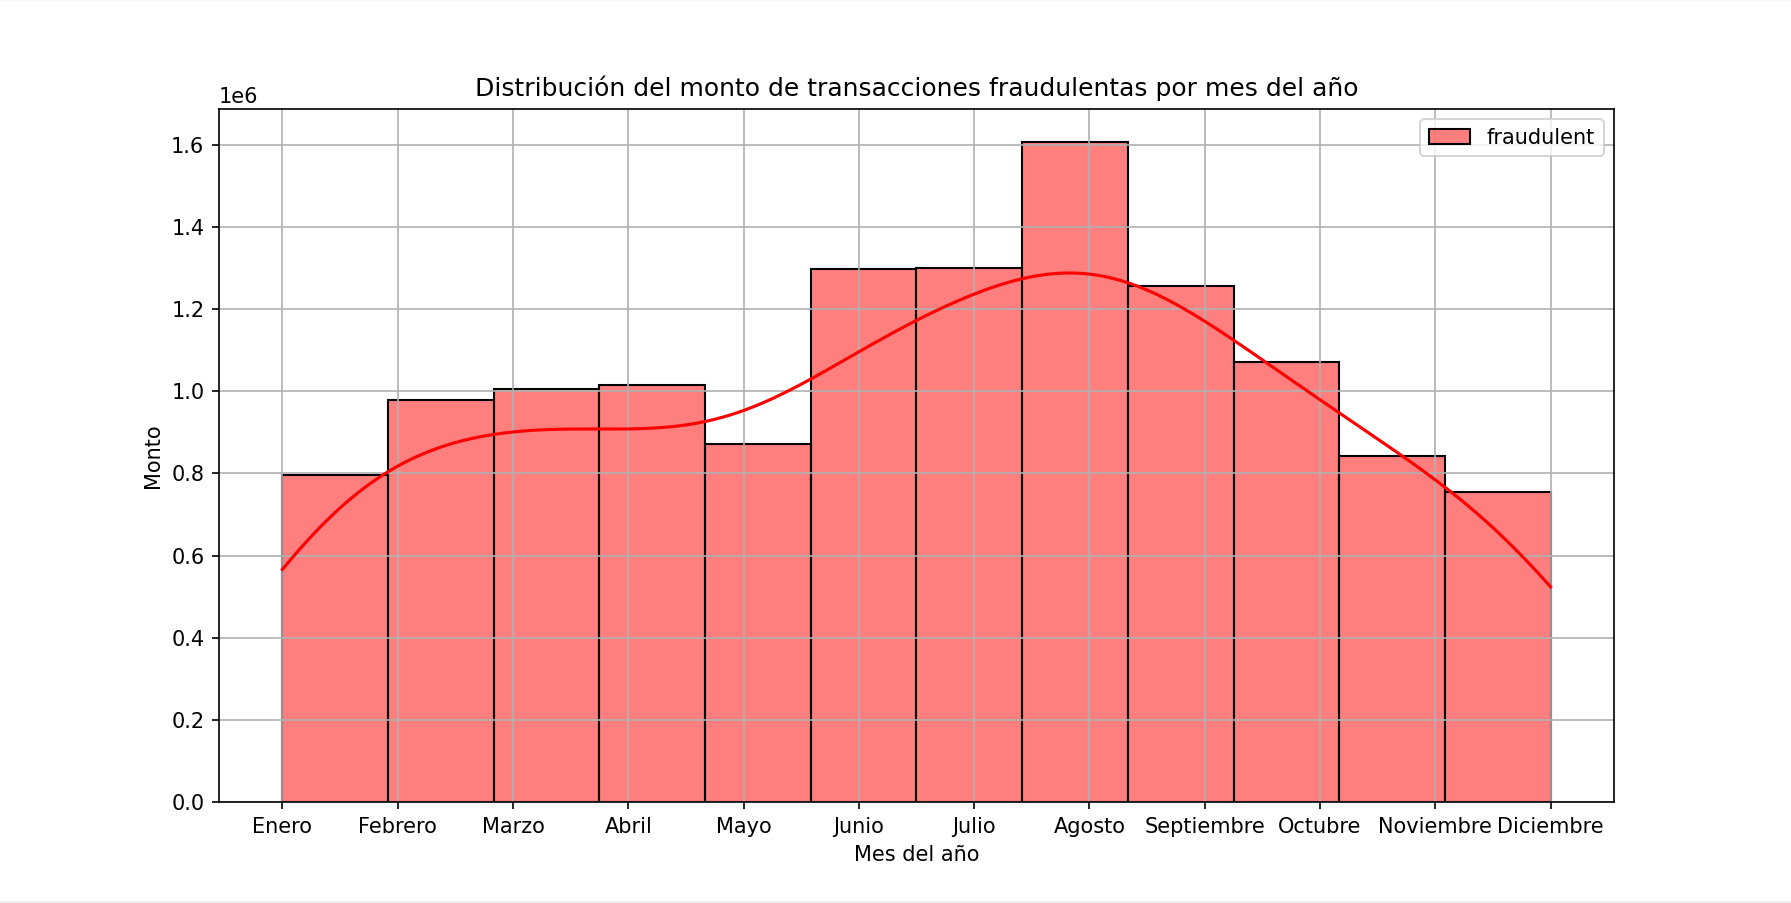
\includegraphics[scale = .3]{IMAGE/histograma5.png}
    \end{center}

    De acuerdo al histograma se puede indicar que los fraudes son más comunes durante la segunda mitad del año, especialmente entre julio y septiembre, lo que podría coincidir 
    con eventos estacionales o períodos específicos de mayor actividad económica o comercial. Después del máximo, los fraudes disminuyen progresivamente hacia diciembre.

\newpage 
\item \textbf{Histograma del monto perdido por mes por transaccines de tipo purchase con estado fraudolenta:}

A continuación se muestra la implementación de este histograma, para que se ejecute vamos a colocar en terminal el comando \textbf{python3 histograma6.py}:

  \begin{lstlisting}[language=Python, caption= Implementación histograma del monto perdido por mes por transaccines de tipo purchase con estado fraudolenta.]
    import pandas as pd
    import matplotlib.pyplot as plt
    import seaborn as sns
    import matplotlib.patches as mpatches
    
    # Cargar el archivo CSV
    data = pd.read_csv('transacciones.csv')
    
    # Crear una nueva columna combinando 'date' y 'time'
    data['transaction_time'] = pd.to_datetime(data['date'] + ' ' + data['time'], format='%d/%m/%Y %H:%M')
    
    # Filtrar transacciones fraudulentas de tipo purchase
    fraudulent_purchase_transactions = data.loc[(data['status'] == 'fraudulent') & 
                                                (data['transaction_type'] == 'purchase')].copy()
    
    # Extraer el mes de la columna 'transaction_time'
    fraudulent_purchase_transactions['month'] = fraudulent_purchase_transactions['transaction_time'].dt.month
    
    # Añadimos un estilo a la gráfica
    sns.set(style="whitegrid")
    
    # Se define y se crea la gráfica
    plt.figure(figsize=(10, 6))
    colors = ["#FF6F61"]
    
    # Crear el histograma con el monto por mes
    sns.histplot(
        data=fraudulent_purchase_transactions,
        x='month', 
        weights='amount',  # Aquí el peso será el monto de la transacción
        bins=12,  # Una barra por cada mes
        color=colors[0],
        edgecolor='black'
    )
    
    # Títulos y etiquetas
    plt.title('Monto perdido por mes en transacciones "purchase" fraudulentas', fontsize=16, fontweight='bold')
    plt.xlabel('Mes del año', fontsize=14)
    plt.ylabel('Monto total de transacciones fraudulentas', fontsize=14)
    
    # Personalizamos los ejes
    plt.xticks(range(1, 13), ['Ene', 'Feb', 'Mar', 'Abr', 'May', 'Jun', 'Jul', 'Ago', 'Sep', 'Oct', 'Nov', 'Dic'], fontsize=12)
    plt.yticks(fontsize=12)
    
    # Cuadrícula en la gráfica
    plt.grid(axis='y', linestyle='--', alpha=0.7)
    
    # Crear la leyenda "Fraudulentas"
    fraud_patch = mpatches.Patch(color='#FF6F61', label='Fraudulentas')
    
    # Guardar la gráfica como imagen en lugar de mostrarla
    plt.legend(handles=[fraud_patch], title='Estado', loc='upper right', fontsize=12)
    plt.tight_layout()
    
    # Guardar la gráfica en un archivo PNG
    plt.savefig('IMAGE/histograma6.png')
    
    plt.show()
\end{lstlisting}

 \begin{center}
    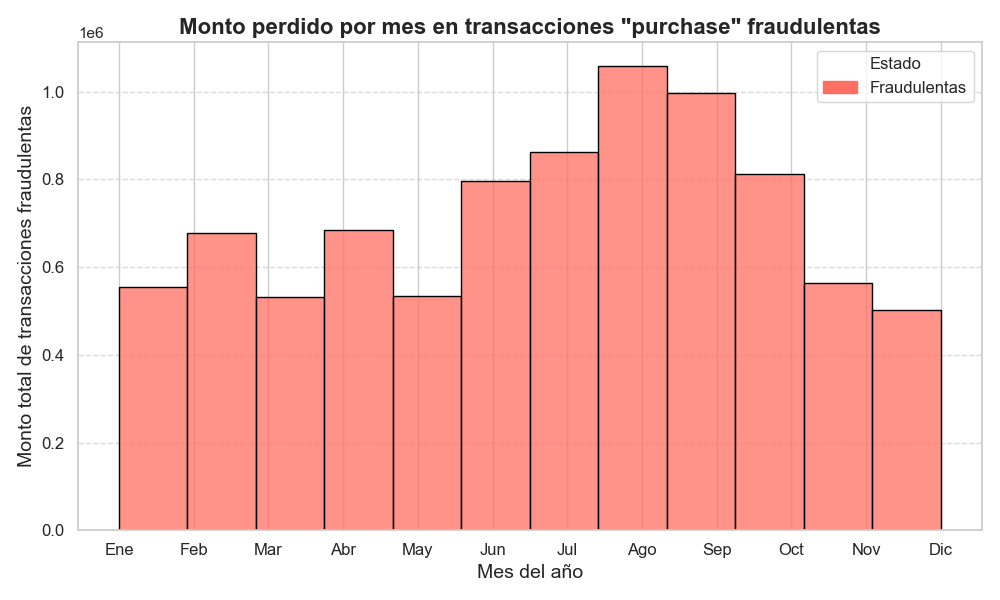
\includegraphics[scale = .3]{IMAGE/histograma6.png}
\end{center}

Se observa que los meses de julio y agosto presentan el mayor número de fraudes, mientras que enero, noviembre y diciembre tienen los niveles más bajos. 
Entre enero y mayo, los montos se mantienen estables, pero a partir de junio se da un aumento significativo que culmina en agosto, seguido de una disminución en septiembre. 
Aunque las compras de fin de año suelen ser altas, noviembre y diciembre registran menos fraudes, lo que podría estar relacionado con medidas preventivas o cambios en el comportamiento de los consumidores.

    
\end{itemize}

{\color{black}\rule{\textwidth}{1.5pt}}

\end{document}